\documentclass[border=6pt]{standalone}
\usepackage{amsmath, amssymb}
\usepackage{tikz}
\begin{document}
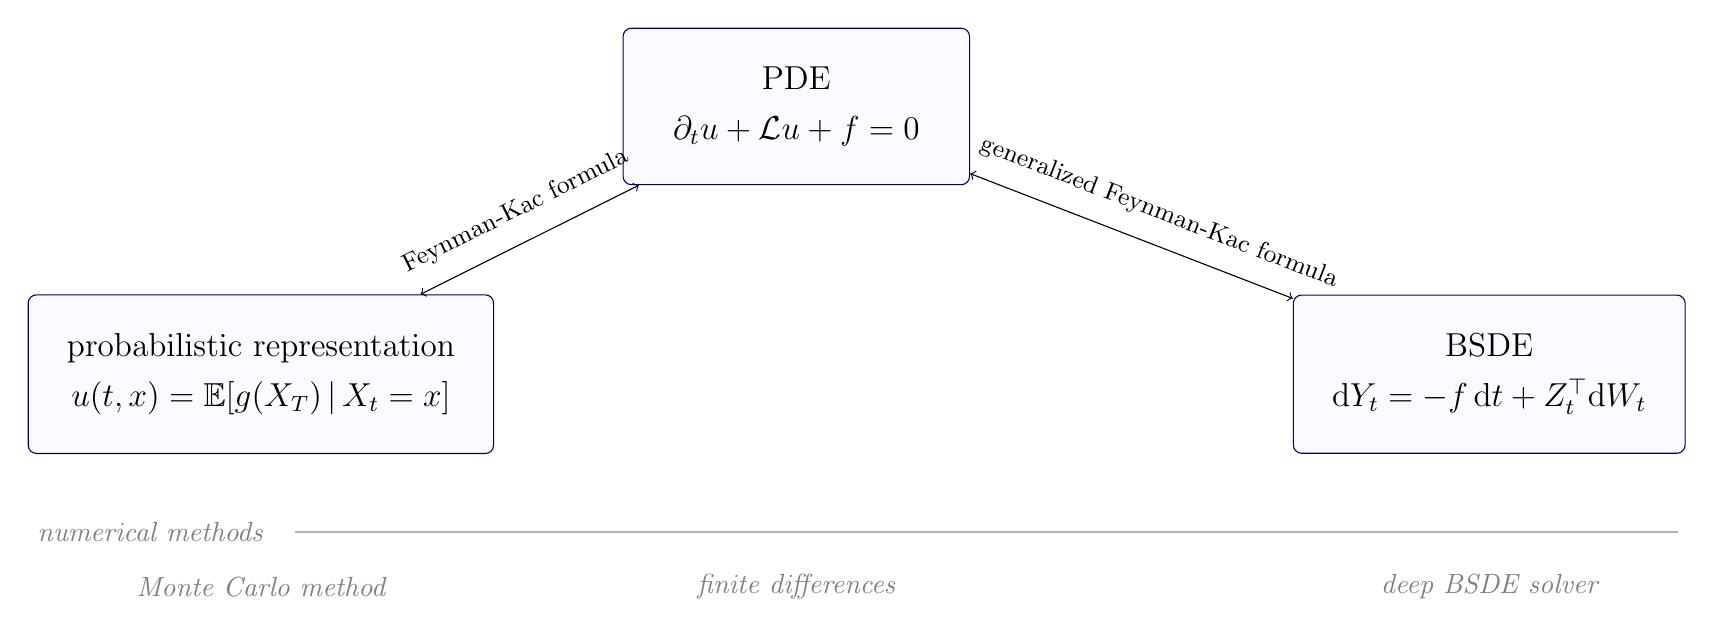
\begin{tikzpicture}[
  box/.style={draw=blue!50!black, fill=blue!2!white, rounded corners=3pt,
    align=center, inner sep=14pt, minimum height=1.8cm, minimum width=4.4cm,
    font=\large},
  meth/.style={font=\itshape, text=black!50, align=center},
  thlab/.style={above=4pt, sloped, font=\small}]
\node[box] (prob) at (0,0)
  {probabilistic representation\\[4pt]$u(t,x) = \mathbb E\!\left[g(X_T)\,\middle|\,X_t = x\right]$};
\node[box] (pde) at (6.8,3.4)
  {PDE\\[4pt]$\partial_t u + \mathcal L u + f = 0$};
\node[box] (bsde) at (15.6,0)
  {BSDE\\[4pt]$\mathrm dY_t = -f\,\mathrm dt + Z_t^{\top}\mathrm dW_t$};
\draw[<->] (prob) -- (pde)
  node[thlab, midway] {Feynman-Kac formula};
\draw[<->] (pde) -- (bsde)
  node[thlab, pos=0.55] {generalized Feynman-Kac formula};

\node[meth, anchor=west] (nm) at (prob.west |- 0,-2.0) {numerical methods};
\draw[gray!60, thick] ([xshift=8pt]nm.east) -- (18.0,-2.0);
\node[meth] at (0,-2.7) {Monte Carlo method};
\node[meth] at (6.8,-2.7) {finite differences};
\node[meth] at (15.6,-2.7) {deep BSDE solver};
\end{tikzpicture}
\end{document}
